%        File: branching_times.tex
%     Created: Mon Jul 06 09:00 AM 2009 C
% Last Change: Mon Jul 06 09:00 AM 2009 C
%
\documentclass[letterpaper,10pt]{article} 
\usepackage[pdftex]{color,graphicx} 
\usepackage{amsmath, amsfonts, amssymb, latexsym, inputenc, moreverb, wrapfig, subfigure, array, lscape, setspace, cite}
\usepackage[pdftex, colorlinks]{hyperref}
\newcommand{\ud}{\mathrm{d}} 
\newcommand{\degree}{$^{\circ}$}
\newcommand{\tb}[1]{\textcolor{blue}{#1}} 
\newcommand{\E}{\text{E}}

%\usepackage{fullpage} %% 1 inch margins by default
%\usepackage{pslatex}  %% use normal postscript fonts (like times new roman)

\title{Calculating the Time until Branching:\\ A Sketch of the Process}
\author{Carl Boettiger}
\begin{document}
\maketitle
\section{Introduction}
Our calculation of the time until branching occurs consists of the following approach.  The first requirement for branching to occur is the existence of two mutually invasible populations separated by an adaptive minimum, that is $s(y,x) >0$, $s(x,y)>0$ and $\partial^2_y s(y,x)>0$.  The minimum (curvature condition) is provided by a singular point of the branching type, which also assures us that there will be some pairs $(y,x)$ near each other $|y-x| \sim o(\sigma_{\mu})$.  These points define a coexistence region in the pairwise invasibility plot, which we denote $P_2$.  A mutant enters this region by ``jumping the gap'' from the line $y=x$ into the coexistence region.  This gap diminishes in width as the resident trait $x$ nears the branching point, where the gap vanishes all together.   This criterion can be evaluated directly at regular intervals throughout the simulation.  

Most often this condition will arise only transiently -- a single mutant satisifying the conditions but soon lost to drift.  Hence our second requirement must be that the mutant successfully entering the coexistence region then proceeds to survive drift.  Defining this second condition rigorously is less straight-forward.  For large populations, the probability of survival may be well approximated by the Galton-Watson branching process.  In theory, this probability can be converted into an expected waiting time in a straight-forward manner.  In simulation, this is insufficent, as we want to identify the actual waiting time we need more than a probability -- we need to indentify which populations actually survive.  If selection is strong, we may hope to identify which populations have effectively survived drift by establishing some low-density threshold at which we declare the population successful.  Of course, this introduces a discrepancy in the definition of waiting time, as the theory calculates the time until a successful mutant occurs, while the simulation lags behind by the time required to go from one individual to the threshold size.  

If selection is strong, we can set this threshold quite low, and more importantly, the time to reach the threshold will be quite small compared to the time spent waiting for the mutation, and theory and simulation should match reasonably well.  This latter observation is particularly convenient in that our calculation shouldn't depend much on the choice of threshold, as once the mutant establishes several clones the probability of survival quickly asymptotes to unity.  If selection is weak, we are not so fortunate.  Even relatively large mutant populations may be at substantial risk to extinction by drift, and this extinction probability will depend quite strongly on the particular choice of threshold.  As selection becomes nearly neutral, no threshold may exist that can guarentee the persistence of the mutant.  

In each case, the persistence of the resident must also be considered, as it is also protected by a selection coefficient when rare which may be weaker than that of the mutant (depending on whether the mutant has occurred closer to or farther from the branching point).  If only weakly protected, it too can be lost to drift.  For the moment, let us consider only the case of strong selection, where a small, arbitrary threshold can reasonably guarentee the success of branching.  Later we will want to quantify the meaning of strong, relative to the influence of drift.  For now, it suffices that such a notion exists, and we need only focus on the first two steps -- a mutant occurs and survives drift with probability given by its selective coefficent, to have a reasonable approximation of the waiting time between simulation and experiment.   

The loss of a mutant in the coexistence region even after invading a significant fraction of the population does not preclude branching.  The population may continue to approach the branching point where such mutations are more common (do they have stronger selection too?)  Even in the purely neutral case, the dimorphism may persist long enough for a new mutant to arise.  This allows the populations to take another mutational steps apart, where selection may be strong enough to protect the dimorphism.  The ability for larger populations to be able to survive drift long enough for this to occur may allow them to branch in face of weak selection where a smaller population would fail.  

(A resource kernel that is similar in width to the competition kernel but very wide compared to the mutational step size may approach the branching region only by drift -- fixing weakly deleterious mutations.  )

\section{Calculation}
The probability of such a mutant occurring in our monomorphic population of trait $x$ is given by the probability that any mutant occurs (given by the population size, approximately $K(x)$ at equilibrium, times the birth rate $b(x)$ times the mutation rate $\mu$) times the probability that the mutation lies on the opposite side of the coexistence boundary, which we denote as $\phi(x)$ and $\psi(x)$, which is $\phi(x)$ reflected across the line $y=x$.  This depends on the mutational kernel, $M(y,x)$ which gives the probability that a mutant arising from a resident population of trait $x$ bears trait $y$ that falls withing the coexistance region as follows:

\begin{equation*}
\int_{-\infty}^{\phi(x)} M(y,x) \ud y + \int_{\psi(x)}^{\infty} M(y,x) \ud y 
\end{equation*}
Without loss of generality let us assume that the singular strategy $x^* = 0$ and that we start from some trait value $x_0 > x^*$.  Additionally, let us we assume $M(y,x)$ is Gaussian in $y-x$ with mean 0 and variance $\sigma_{\mu}^2$. However, we do not wish to consider all such mutants $y$, but only those that survive.  We multiply the probability of a mutant having trait $y$, $M(y,x)$, times the probability that is survives drift.  This probability we quote from the Galton-Watson branching process, $1-\tfrac{d(y,x)}{b(y,x)}$.  Taking as our model the individual birth $b$ and death $d$ rates to be:

\begin{align}
b(y,x) &= r\\
d(y,x) &= r\frac{C(y,x)K(x)}{K(y)}
\end{align}

where $K$ is a Gaussian kernel with mean $x^*$, $K(x^*) = K_0$ and variance $\sigma^2_k$ and $C(y,x)$ a Gaussian kernel in $y-x$ with mean $0$, $C(0) =1$ and variance $\sigma^2_c$. Using this choice of model, the probability of surviving branching is

\begin{equation}
1-\frac{C(y,x)K(x)}{K(y)} := S(y,x)
\label{S}
\end{equation}

which we denote as $S(y,x)$ as indicated. Hence we modify our integral to consider all mutants $y < x^*$ which occur with probability $M(y,x)$ and then survive with probability $S(y,x)$, and write down the rate $P(x)$ at which a mutant which leads to branching occurs from our monomorphic population with trait $x$:

\begin{equation}
P(x) := r \mu K(x)\left( \int_{-\infty}^{\phi(x)} M(y,x) S(y,x) \ud y + \int_{\psi(x)}^{\infty} M(y,x) S(y,x) \ud y  \right)
\label{MSerf}
\end{equation}

Though a little cumbersome, this can be written in nearly closed form (using the error function). For our particular model $s(y,x)$, we can write the boundaries $\phi(x)$ and $\psi(x)$ as 

\begin{align}
\phi(x) = x\frac{\frac{\sigma_k^2}{\sigma_c^2}+1}{\frac{\sigma_k^2}{\sigma_c^2}-1} \nonumber \\
\psi(x) = x\frac{\frac{\sigma_k^2}{\sigma_c^2}-1}{\frac{\sigma_k^2}{\sigma_c^2}+1}
\label{phipsi}
\end{align}
Then, given a starting condition $x_0$, we can determine the expected trait $x$ at time $t$ of a monomorphic resident population by integrating the canonical equation,

\begin{equation}
\frac{\ud x}{\ud t} = \frac{1}{2} \mu \sigma_{mu}^2 N^*(x) \partial_y s(y,x)
\end{equation}

which for our model is  
\begin{equation}
\frac{\ud x}{\ud t} = \frac{-x}{2\sigma_k^2} r \mu \sigma_{\mu}^2 K(x) 
\end{equation}
While no closed form solution exists for $x(t)$ in this case, if we assume $x_0 \ll \sigma_k$ then to good approximation we can view $K(x)$ to be constant over the interval and take our path to be:

\begin{equation}
x(t) = x_0 \exp\left( -r \mu \sigma_{\mu}^2 K_0 t/\sigma_k^2\right)
\end{equation}

Using this mean path, we can write down an approximation for the rate of a branching mutant occurring as a function of time, $P(x(t))$.  Using this time dependent rate, the probability of not branching after time $T$ is simply $\exp\left( - \int_0^T P(t)\ud t \right)$.  One minus this is the probability branching by time $T$; i.e. the cumulative density function, hence the probability density function for the waiting time is:

\begin{equation}
\Pi(T) = P(x(T)) \exp\left( -\int_0^T P(x(t)) \right)
\label{pdf}
\end{equation}

and the expected time until branching is $\int_0^{\infty} T \Pi(T) \ud T$. This is our first analytic approximation.  

\begin{figure}
\begin{center}
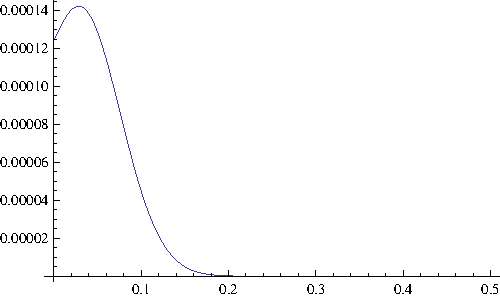
\includegraphics[width=.9\textwidth]{myp}
\caption{The function $P(x)$ shown over the domain from $x_0 = 0.5 $ to the branching point, 0.}
\end{center}
\end{figure}

\begin{figure}
\begin{center}
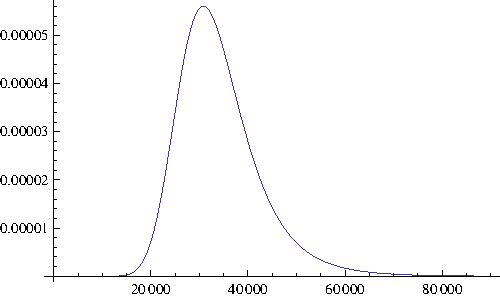
\includegraphics[width=.9\textwidth]{mywaiting}
\caption{The distribution of waiting times from this approximation.  This distribution has a mean of 34130, and variance $4.4\cdot 10^7$.}
\end{center}
\end{figure}

\begin{figure}
\begin{center}
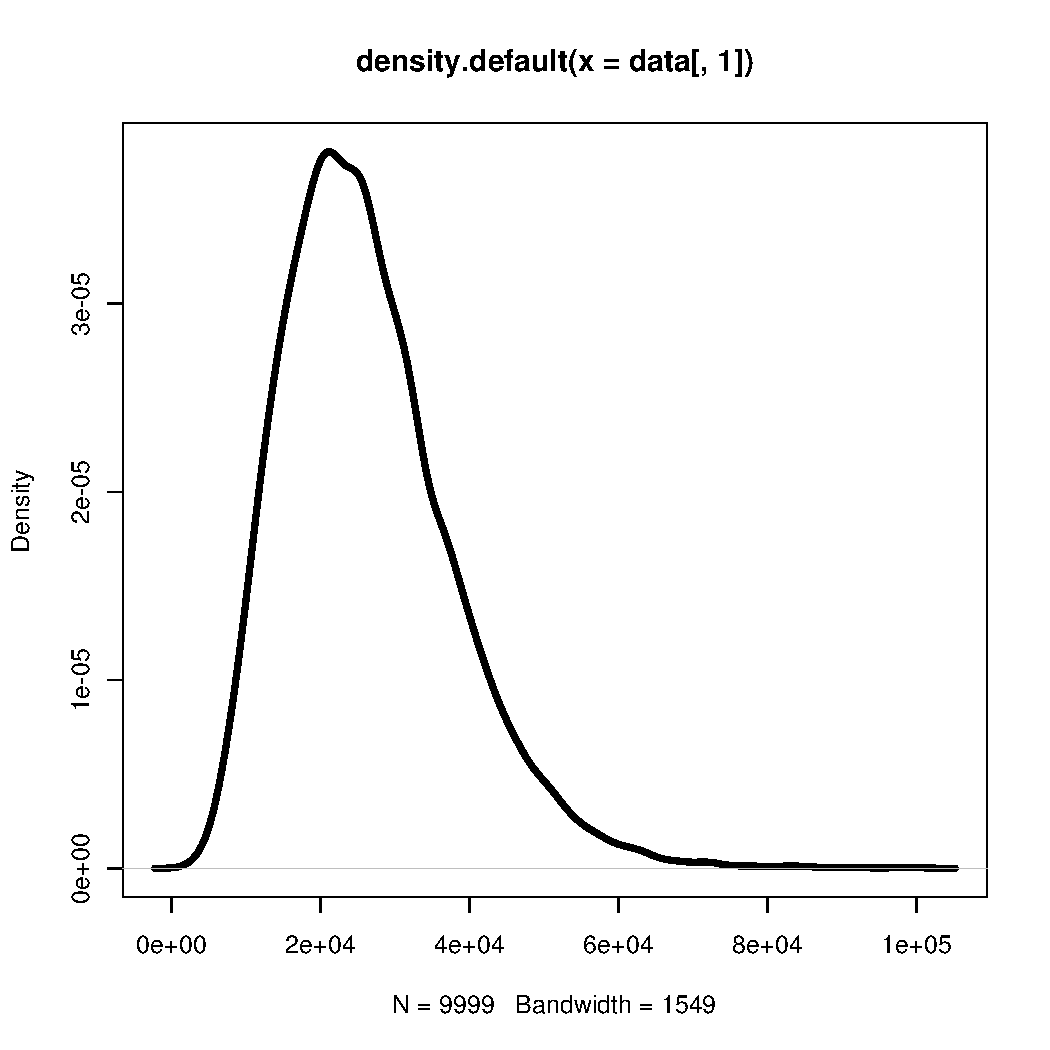
\includegraphics[width=.9\textwidth]{waittimes}
\caption{The distribution of waiting times from the simulation (smoothing by kernel density estimation).   This distribution has a mean of 26330, and variance $12.9\cdot 10^7$.}
\end{center}
\end{figure}


\begin{multline*}
P(x) = \frac{1}{2} \left(1+ {Erf}\left[\frac{x}{\sqrt{2} \sqrt{\sigma_{\mu}^2}}\right]\right)-\\
\Biggl(e^{\frac{\sigma_{\mu}^2  {\sigma_{c}^2} x^2}{2  {\sigma_{k}^2} ( {\sigma_{c}^2}  {\sigma_{k}^2}+\sigma_{\mu}^2 (- {\sigma_{c}^2}+ {\sigma_{k}^2}))}}  {\sigma_{c}^2} \Biggl(\sqrt{\frac{ {\sigma_{k}^2} ( {\sigma_{c}^2}  {\sigma_{k}^2}+\sigma_{\mu}^2 (- {\sigma_{c}^2}+ {\sigma_{k}^2})) x^2}{\sigma_{\mu}^2  {\sigma_{c}^2}}}+\\
\sqrt{\frac{1}{\sigma_{\mu}^2}+\frac{1}{ {\sigma_{c}^2}}-\frac{1}{ {\sigma_{k}^2}}}  {\sigma_{k}^2} x  {Erf}\left[\frac{\sqrt{-\frac{(\sigma_{\mu}^2+ {\sigma_{c}^2})^2  {\sigma_{k}^2} x^2}{\sigma_{\mu}^2  {\sigma_{c}^2} (\sigma_{\mu}^2 ( {\sigma_{c}^2}- {\sigma_{k}^2})- {\sigma_{c}^2}  {\sigma_{k}^2})}}}{\sqrt{2}}\right]\Biggr)\Biggr)/\left(2 ( {\sigma_{c}^2}  {\sigma_{k}^2}+\sigma_{\mu}^2 (- {\sigma_{c}^2}+ {\sigma_{k}^2})) \sqrt{\frac{x^2}{\sigma_{\mu}^2}}\right)
\end{multline*}
\end{document}


